\subsection{光滑解的爆破}\label{sec:conservation-smooth-blowup}

如上所述, 本章的主要目的是研究具有不连续解的偏微分方程. 现在已做好准备, 可以说明守恒律的不连续解如何由连续解发展而来.

\subsubsection{单个守恒律}\label{subsec:scalar-conservation-blowup}

考虑如下形式的单个守恒律
\begin{equation}\label{eq:scalar-conservation-law-quasilinear}
u_t+f'(u)u_x=0.
\end{equation}
这里假设 $f$ 足够光滑. 方程 \eqref{eq:scalar-conservation-law-quasilinear} 的特征曲线必须满足
\begin{equation}\label{eq:scalar-conservation-characteristic-ode}
\hat x'(t)=f'(u(\hat x(t),t)).
\end{equation}


由这一关系, 可对单个守恒律得到以下很强的结果.

\begin{Theorem}
\label{thm:scalar-constant-characteristics}
单个守恒律 \eqref{eq:scalar-conservation-law-quasilinear} 的任意 $C^1$ 解沿特征线为常数. 因而, 方程 \eqref{eq:scalar-conservation-law-quasilinear} 的特征曲线是直线.
\end{Theorem}

\begin{Proof}
利用 \eqref{eq:scalar-conservation-law-quasilinear} 和 \eqref{eq:scalar-conservation-characteristic-ode}, 得到
\begin{equation}\label{eq:scalar-solution-constant-along-characteristics}
\dfrac{\mathrm{d}}{\mathrm{d}t}u(\hat x(t),t)=u_x\hat x'+u_t=u_xf'(u)+u_t=0.
\end{equation}
因此
\begin{equation}\label{eq:scalar-characteristic-constant-value}
u(\hat x(t),t)=C
\end{equation}
其中 $C$ 为常数. 所以由 \eqref{eq:scalar-conservation-characteristic-ode} 可得
\begin{equation}\label{eq:scalar-straight-characteristic-line}
\hat x(t)=kt+\hat x(0),
\end{equation}
其中 $k$ 是常数 $k:=f'(C)$.
\end{Proof}

\begin{figure}[H]
\centering
\includegraphics[page=84,pagebox=cropbox,trim=94.00bp 403.88bp 93.56bp 69.00bp,clip,width=.78\linewidth]{../input/source/An Introduction to Partial Differential Equations.pdf}
\caption{通过特征线定义解.}\label{fig:characteristic-construction}
\end{figure}

为了解这对 Cauchy 问题的解一般意味着什么, 重点考察 Burgers 方程
\begin{equation}\label{eq:burgers-characteristic-cauchy-equation}
u_t+uu_x=0
\end{equation}
及初始条件
\begin{equation}\label{eq:burgers-characteristic-cauchy-data}
u(x,0)=u_0(x).
\end{equation}
注意, 特征方程化为
\begin{equation}\label{eq:burgers-characteristic-slope}
\hat x'(t)=u(\hat x(t),t).
\end{equation}


因此, 初始数据给出了从 $x$ 轴出发的特征射线的斜率. 对某些初始数据, 这就给出一种"求解" Cauchy 问题的方法. 只需沿 $x$ 轴, 按初始数据决定的斜率画出特征射线, 并令解沿特征线取相应初始数据的值 (参见 Figure~\ref{fig:characteristic-construction}).

可惜, 一些不连续初始数据的简单例子表明, 这一过程很容易失效. Figure~\ref{fig:characteristic-gap} 显示, 对应于阶跃函数的初始条件, 存在一个区域, 从初始数据出发的任何特征线都未经过它; 上述过程不能确定这一区域内的解. 如下文将看到的, 在这种情形下可以确定一个连续解, 称为稀疏波或扇形波.

然而, Figure~\ref{fig:characteristic-overlap} 中的问题更为困难. 对递减的阶跃函数, 特征线相互交叠. 由于解不能是多值的, 必须得出结论 (根据 Theorem~\ref{thm:scalar-constant-characteristics}): 解不可能光滑. 对这种初始数据, 必须发展不连续解, 即"激波"的理论.

\begin{figure}[H]
\centering
\includegraphics[page=85,pagebox=cropbox,trim=95.00bp 403.88bp 94.56bp 70.00bp,clip,width=.78\linewidth]{../input/source/An Introduction to Partial Differential Equations.pdf}
\caption{特征线不能确定空白区域内的解.}\label{fig:characteristic-gap}
\end{figure}

\begin{figure}[H]
\centering
\includegraphics[page=85,pagebox=cropbox,trim=95.00bp 168.88bp 94.56bp 297.00bp,clip,width=.78\linewidth]{../input/source/An Introduction to Partial Differential Equations.pdf}
\caption{特征线相互交叠.}\label{fig:characteristic-overlap}
\end{figure}

注意, 在这种情形下将数据光滑化也无济于事; 这只是推迟了问题的出现. 事实上, 以下定理表明, 特征线交叠和奇性的形成是一个普遍的问题.

\begin{figure}[H]
\centering
\includegraphics[page=86,pagebox=cropbox,trim=91.62bp 402.34bp 93.70bp 70.25bp,clip,width=.78\linewidth]{../input/source/An Introduction to Partial Differential Equations.pdf}
\caption{从连续初始数据出发的特征线相交.}\label{fig:continuous-characteristic-crossing}
\end{figure}

\begin{Theorem}
\label{thm:scalar-finite-time-blowup}
若 $f''>0$, 且初始数据 $u_0$ 不是单调递增的, 则方程 \eqref{eq:scalar-conservation-law-quasilinear} 的 Cauchy 问题不存在定义在整个上半平面 $(x,t)\in(-\infty,\infty)\times[0,\infty)$ 上的 $C^1$ 解.
\end{Theorem}

\begin{Proof}
证明仅依赖于如下观察: 若对 $x_1<x_2$ 有 $f'(u_0(x_1))>f'(u_0(x_2))$, 则从 $x_1$ 和 $x_2$ 出发的特征线将在有限时间内相交 (参见 Figure~\ref{fig:continuous-characteristic-crossing}).
\end{Proof}

\subsubsection{$p$ 方程组}\label{subsec:p-system-blowup}

对 $p$ 方程组, 特征曲线不再如此简单, 因而使用更多分析技巧证明爆破. 利用在状态空间中改用 Riemann 不变量坐标得到的方程组的对角形式 \eqref{eq:p-system-diagonal-first}, \eqref{eq:p-system-diagonal-second}. 由于 Theorem~\ref{thm:p-system-characteristic-invariants} 表明 $\rho_1$ 和 $\rho_2$ 沿各自的特征曲线为常数, 只要解保持 $C^1$, 就不能期望它们变为无界. 但若考察斜率 $\rho_{1,x}$ 和 $\rho_{2,x}$ 的演化, 就可能出现问题. 因此, 将 \eqref{eq:p-system-diagonal-first} 和 \eqref{eq:p-system-diagonal-second} 对 $x$ 求导, 得到
\begin{equation}\label{eq:p-system-first-slope-equation}
\rho_{1,xt}+\hat\lambda(\rho_1-\rho_2)\rho_{1,xx}=-\hat\lambda'(\rho_1-\rho_2)(\rho_{1,x}^2-\rho_{1,x}\rho_{2,x}),
\end{equation}

\begin{equation}\label{eq:p-system-second-slope-equation}
\rho_{2,xt}-\hat\lambda(\rho_1-\rho_2)\rho_{2,xx}=-\hat\lambda'(\rho_1-\rho_2)(\rho_{2,x}^2-\rho_{1,x}\rho_{2,x}).
\end{equation}
乘积项 $\rho_{1,x}\rho_{2,x}$ 引起不便的耦合, 但可用变量变换 $r:=\hat\lambda^{1/2}\rho_{1,x}$, $s:=\hat\lambda^{1/2}\rho_{2,x}$ 消去它们.

作此变换后, 方程组变为
\begin{equation}\label{eq:p-system-weighted-first-slope}
r_t+\hat\lambda(\rho_1-\rho_2)r_x=-\hat\lambda^{-1/2}(\rho_1-\rho_2)\hat\lambda'(\rho_1-\rho_2)r^2,
\end{equation}

\begin{equation}\label{eq:p-system-weighted-second-slope}
s_t-\hat\lambda(\rho_1-\rho_2)s_x=-\hat\lambda^{-1/2}(\rho_1-\rho_2)\hat\lambda'(\rho_1-\rho_2)s^2.
\end{equation}
因此, $r$ 和 $s$ 沿特征线的导数分别与 $r^2$ 和 $s^2$ 成正比. 据此考虑以下引理.

\begin{Lemma}
\label{lem:riccati-finite-time-blowup}
设 $z$ 为常微分方程初值问题
\begin{equation}\label{eq:riccati-positive-coefficient}
z'(t)=a(t)z^2(t),
\end{equation}

\begin{equation}\label{eq:riccati-positive-initial-value}
z(0)=m>0,
\end{equation}
的解, 其中 $0<B\leq a(t)\leq A$. 那么 $z$ 在时刻 $t_c\in((mA)^{-1},(mB)^{-1})$ 变为无穷大 (具有垂直渐近线). 此外, 当 $t<t_c$ 时有估计
\begin{equation}\label{eq:riccati-blowup-bounds}
\dfrac1{A(t_c-t)}<z(t)<\dfrac1{B(t_c-t)}.
\end{equation}

\end{Lemma}

利用这一结果和上面的计算, 可证明

\begin{Theorem}
\label{thm:p-system-finite-time-blowup}
假设
\[
\sup_{x_1,x_2\in\mathbb{R}}\hat\lambda'(\rho_1(x_1,0)-\rho_2(x_2,0))<0
\]
且
\[
m:=\max[\sup_xr(x,0),\sup_xs(x,0)]>0.
\]
令
\[
\begin{aligned}
A&:=-\inf_{x_1,x_2\in\mathbb{R}}\hat\lambda^{-1/2}\hat\lambda'(\rho_1(x_1,0)-\rho_2(x_2,0)),\\
B&:=-\sup_{x_1,x_2\in\mathbb{R}}\hat\lambda^{-1/2}\hat\lambda'(\rho_1(x_1,0)-\rho_2(x_2,0)).
\end{aligned}
\]
那么 $r$ 和 $s$ 至少有一个在 $(mA)^{-1}$ 与 $(mB)^{-1}$ 之间的某个时刻变为无界.
\end{Theorem}

本定理和 Lemma~\ref{lem:riccati-finite-time-blowup} 的证明留给读者作为练习.
